\documentclass[oneside]{scrreprt}

\usepackage[utf8]{inputenc}

\inputencoding{utf8}

\usepackage{blindtext}
\usepackage{graphicx}
\usepackage{abstract}
\usepackage[headsepline]{scrlayer-scrpage}
\usepackage{listings}
\usepackage[hidelinks,bookmarks,urlcolor=uniblue]{hyperref}
\usepackage{mathtools}
%\usepackage{ftnright}
\pagestyle{scrheadings}
\graphicspath{ {./pics/} }
\usepackage{xcolor}
\usepackage{soul}
\usepackage{url}
\usepackage{svg}
\usepackage{amsmath}
\usepackage{xcolor}
\usepackage{doi}
\usepackage{tikz}
\usetikzlibrary{arrows.meta,calc,fadings,backgrounds}
\usepackage{float}
\usepackage{array}

\definecolor{Light}{gray}{.90}
\sethlcolor{Light}

\definecolor{uniblue}{RGB}{0,99,166}
\definecolor{uniwine}{RGB}{246,168,0}
\definecolor{uniwine}{RGB}{167,28,73}
\definecolor{unilightgreen}{RGB}{148,193,84}
\definecolor{unigrey}{RGB}{102,102,102}

\newcommand{\code}[1]{\texttt{\hl{#1}}}

\usepackage[backend=biber,style=chem-acs,bibencoding=utf8]{biblatex}
\DeclareFieldInputHandler{note}{% deletes the unneccessary Publisher/etex entries
  \def\NewValue{}}

\addbibresource{references_zotero.bib}
\title{Implementation of Auxiliary Restraints for Relative Binding Free Energy Calculations in the 'common-core serial-atom-insertion' Framework \texttt{Transformato}}
\author{Supervised by: Univ-Prof. Dr. Stefan Boresch\\Submitted by: \hspace{26mm}Alexander Grasser}
\date{June 2022}
\publishers{Department of Computational Biological Chemistry\\University of Vienna\\
\includegraphics[width=5cm]{Uni_Logo_2016.jpg} }
\subject{Thesis for the title Bachelor of Science in Chemistry}

\automark[chapter]{chapter}
\ihead{Bachelor's Thesis}
\chead{}

\ohead{\headmark}


\RedeclareSectionCommand[pagestyle=scrheadings,beforeskip=0pt]{chapter}






\begin{document}

\begin{titlepage}

\maketitle{}
\end{titlepage}
\section*{Abstract}
    
    For protein-ligand affinity at binding sites, the relative (and absolute) binding free energy is arguably the most important indicator. Traditionally, calculating these energies is done using comprehensive, GPU-assisted "soft-core" modeling. The 'common-core serial-atom-insertion' framework \texttt{Transformato} instead allows to efficiently divide the problem into sequential fragments solvable by traditional MD calculations. However, issues arise when ligands leave the binding site during simulation. This work presents a possible solution by enabling both automatic and manual addition of restraints to the system.
\vspace{\fill}
\section*{Notes}
\noindent\begin{minipage}{0.7\textwidth}
The data compiled for this thesis may be accessed at GitHub under \url{https://github.com/agrass15268/AuxiliaryRestraintsTransformato/tree/data} or with the QR - Code to the right.
\end{minipage}
\hspace{0.1\textwidth}
\begin{minipage}{0.2\textwidth}
\includesvg[height=2cm]{qrcode}
\end{minipage}
 
\vspace{1cm}

\noindent\begin{minipage}{0.7\textwidth}
Source code and packaged versions of the \texttt{Transformato} package may be retrieved from its GitHub repository at  \url{https://github.com/wiederm/transformato} or with the QR - Code to the right.
\end{minipage}
\hspace{0.1\textwidth}
\begin{minipage}{0.2\textwidth}
\includesvg[height=2cm]{qrcodetrafo}
\end{minipage}
\newpage

\begingroup
\let\clearpage\relax
\renewcommand\contentsname{Table of Contents}
\tableofcontents
\addtocontents{toc}{~\hfill\textbf{Page}\par}
\endgroup
%\renewcommand{\thefootnote}{\Roman{footnote}}
\chapter{Introduction}
Almost since the inception of computer-assisted molecular modeling, a significant focus has been on the interaction of pharmaceutically active biomolecules. Designing and testing lead compounds to catalyze or inhibit biochemical processes is a major focus of research and development efforts, and a comparatively easy-to-access parameter with nevertheless good predictive capabilities has long been the relative binding free energy difference, especially with recent advancements in computational power \cite{cournia_relative_2017}.

\begin{figure}[h]
    \begin{center}
        
    
    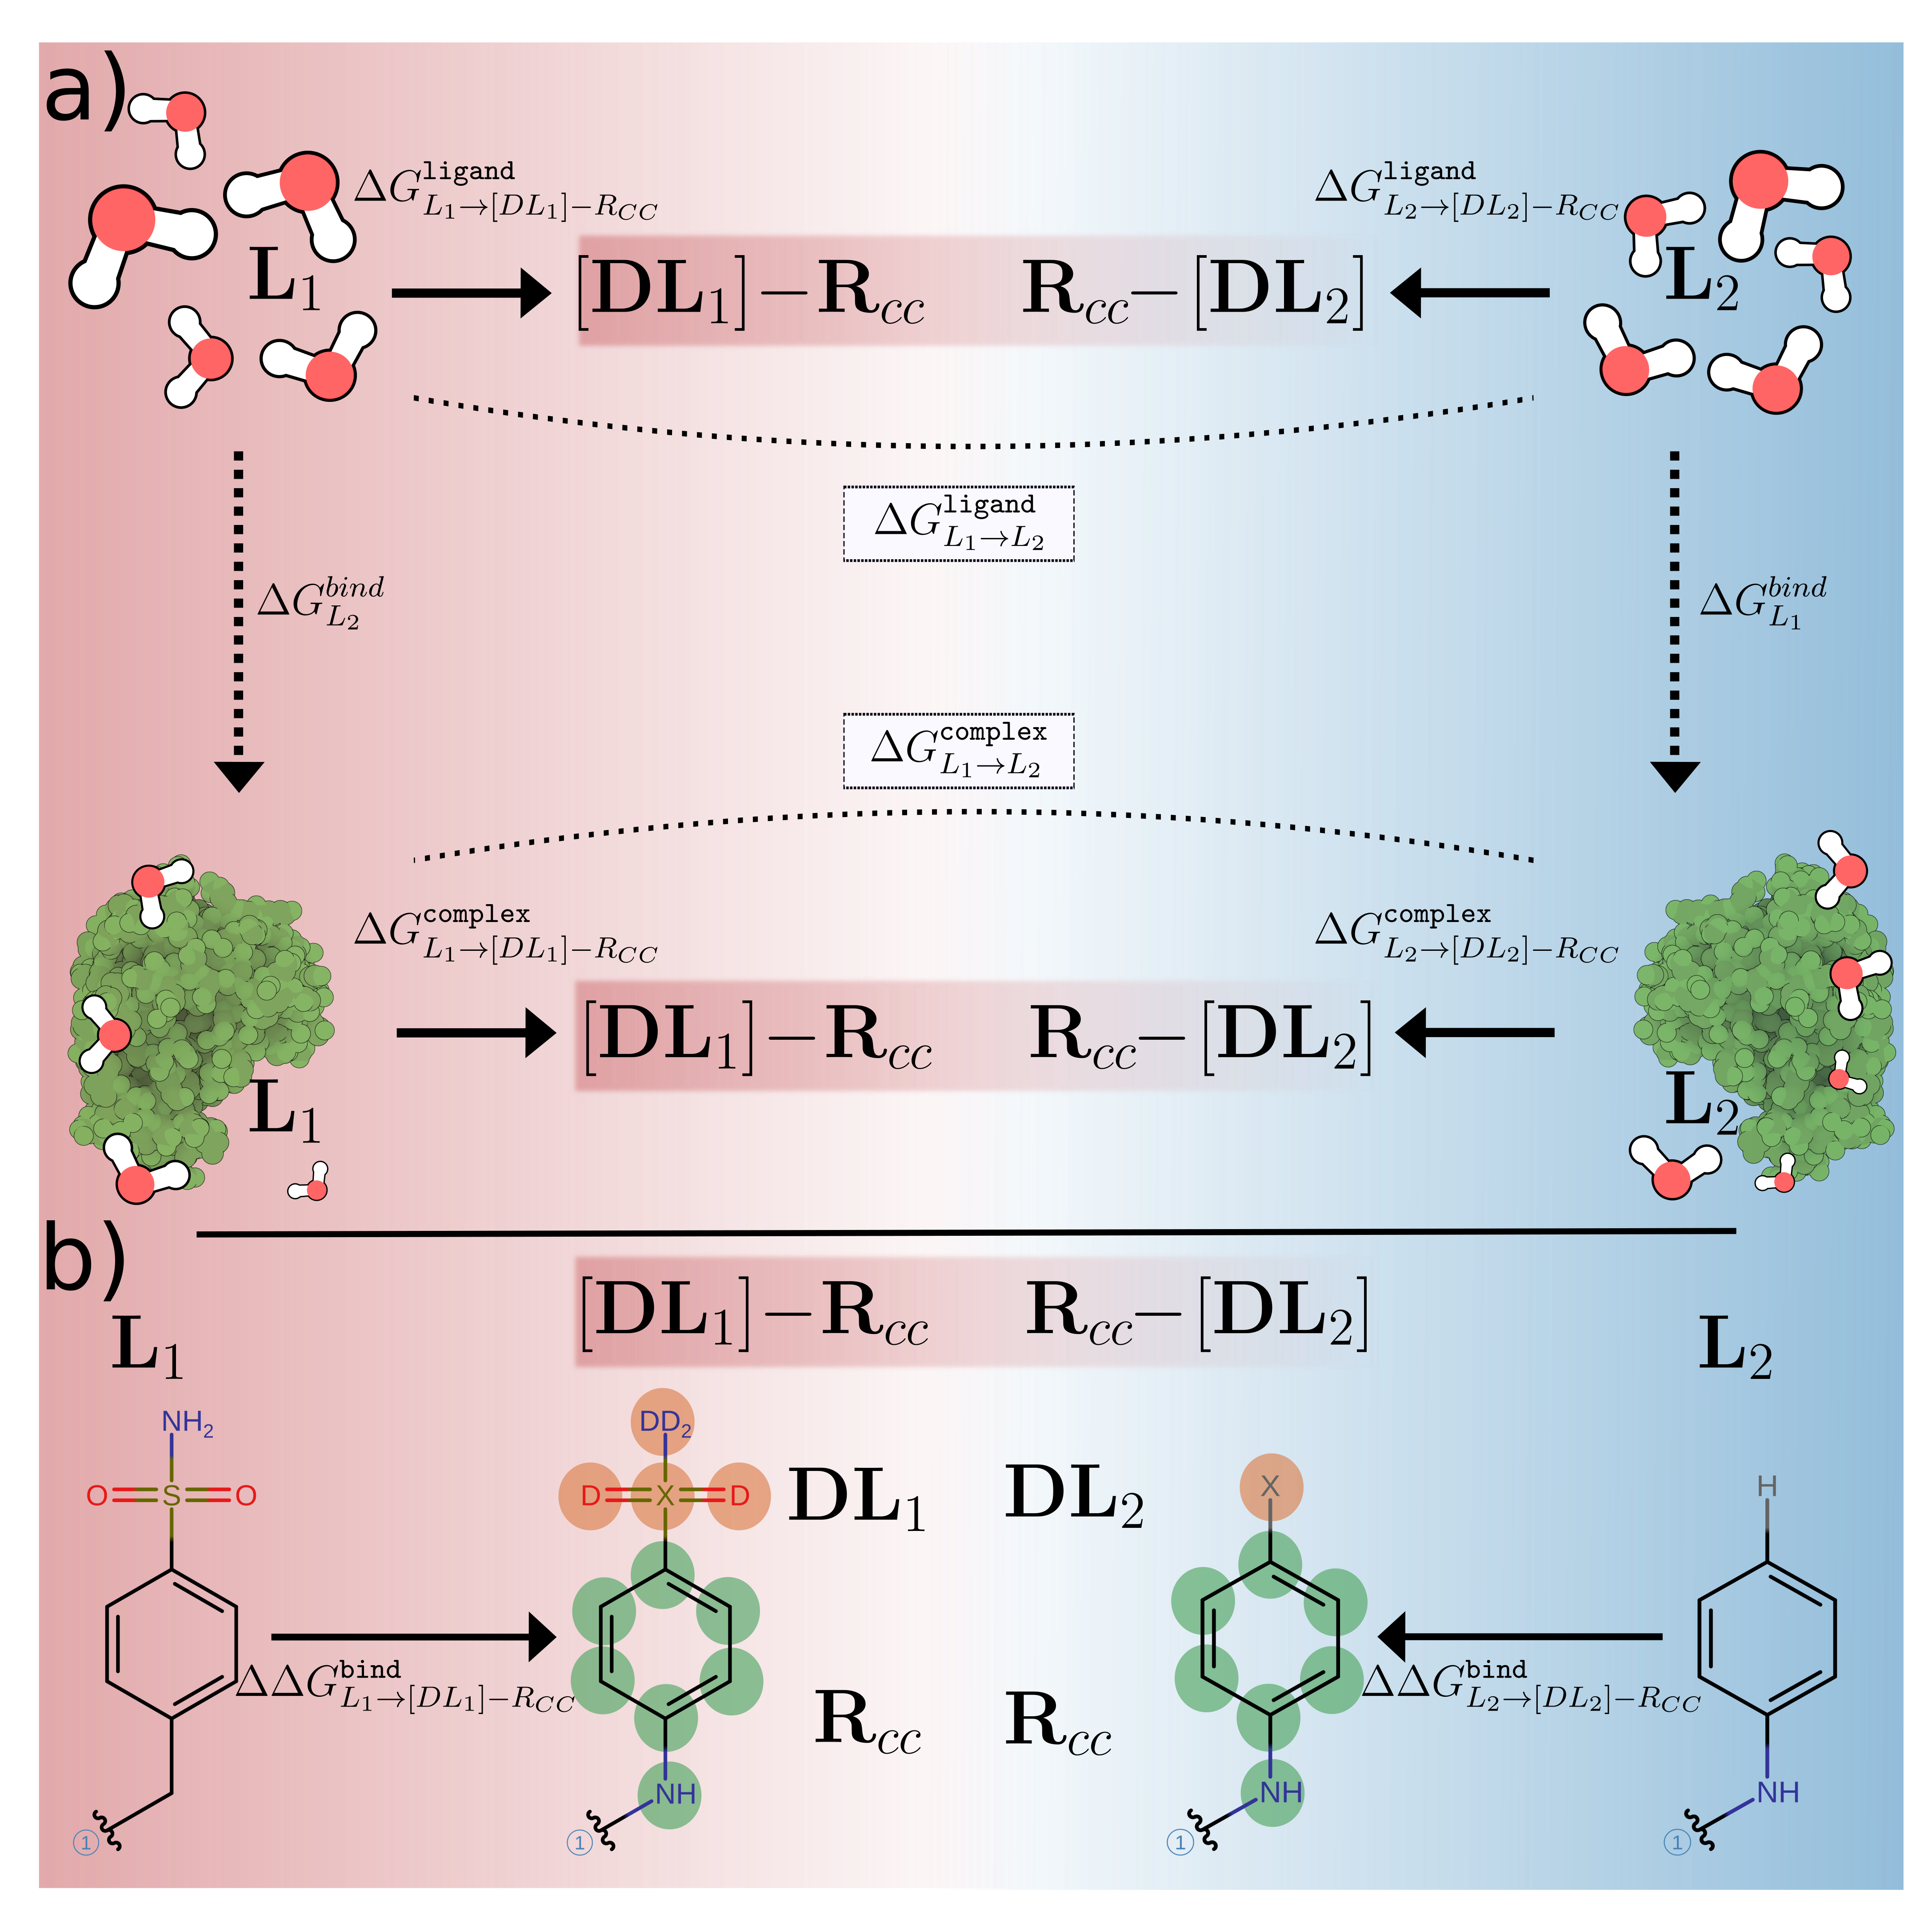
\includegraphics[width=0.7\textwidth]{FESvsTrafo.png}
    \end{center}
    \caption{Overview of \texttt{Transformato}'s workflow}
    a) Comparison between alchemical transformations undertaken by traditional FES (dotted arrows) and the approach taken by \texttt{Transformato} (bold arrows). b) Example mutation path taken to transform two simple molecules into their common core. Green represents the common core, red those atoms that undergo mutation effects or are transferred into dummy atoms.
    \label{fig:fesvstrafo}
\end{figure}

Recently, the package \texttt{Transformato} was introduced by Karwounopoulos, Wieder, Braunsfeld, and Boresch\cite{Karwou2022Jun,braunsfeldImplementationTestingCHARMM,Wieder2022Jun}, implementing a novel approach to bypass these problems. Being a python package, \texttt{Transformato} is easy to install, use, and modify to adapt to system-specific challenges or support different MD engines. Instead of full alchemical transformations of one compound into the other, it instead relies on computing a \emph{common core} (CC) between the two physical endpoints. Summing up the energy differences between the CC and the endstates allows calculation of the free energy difference between the endstates themselves (see Fig. \ref{fig:fesvstrafo}).



With this method, atoms outside the common core are transformed into so-called \emph{dummy atoms}, a term for particles that, while still present in the simulated system, no longer have nonbonded interactions and are only kept in place by weak bonded interactions. If handled properly, these do not contribute to the calculated free energies\cite{fleckDummyAtomsAlchemical2021}.

These dummy atoms are introduced along several intermediate states, alongside various levels of scaling of nonbonded interactions. These intermediate states are then analysed using the \emph{multistate Bennett Acceptance Ratio}\cite{shirts_statistically_2008} (mBAR), an expanded version of Bennet's acceptance ratio\cite{Bennett1976Oct}, ideally giving a close approximation of the sought relative free energy $\Delta\Delta G$. However, mBAR requires topological overlap between the various intermediate states - a problematic proposition if the ligand is liable to abscond its binding site during the simulation timeframe. To prevent this, an additional module \code{restraints.py} was developed and integrated into transformato. It allows the user to either request automatic restraints or define their own. These restraints as implemented act upon the center of mass of the selected ligand atoms, restraining them to their original positions.

To suit a variety of sampling needs, both harmonic and flat-bottomed energy potentials may be used as energy functions for these restraints. This way, a ligand may be specifically allowed to sample the entire binding site without being constrained, yet never leave it. This allows for better sampling and longer runtimes even at increased temperatures, without fear of losing the ligand.
\chapter{Theory}

\section{Theoretical Background}
Simulating the dynamics of (bio-)chemical processes (referred to as \emph{Molecular Dynamics} (MD)) in their entirety can be divided into two classes: calculations utilizing \emph{Quantum Mechanics} (QM), where interactions are calculated according to Schrödinger's Equation, and \emph{Molecular Mechanics} (MM), where calculations instead use a simplified mass-charge-force model to calculate potential energies. While there is no doubt that methods utilizing QM can deliver more accurate results (especially if using "pure" QM and not using semi-empirical methods), computational costs prohibit their use in large biological systems ("large" in this context referring to even just a single protein and its ligand) \cite{cournia_relative_2017}. Thus, for free energy calculations of the sort \texttt{transformato} is designed to accomplish, QM methods are unsuitable - which leaves Molecular Mechanics.

Which is not to say that QM has no place in MD simulations. QM is routinely used to improve geometries and improve calculation precision, with QM/MM methods existing that allow MM and QM calculations to run in the same MD simulation, using QM to calculate the necessary forces for the MM simulation, enhancing accuracy while limiting computational costs. Perhaps most importantly, the force fields used for MD simulations start out as QM calculations that are then fitted to experimental data \cite{vanommeslaeghe_charmm_2010}. Still, for this thesis, only MD based on Molecular Mechanics was used.



\subsection{Basics of Molecular Dynamics Modeling}

Since the discovery of cells, the inner workings of biological systems have always been a mystery science has raced to solve. While of course, physical methods have allowed some degree of monitoring biochemical processes, these have significant limits - most glaringly being limited to physically-present structures. With Molecular Dynamics (MD) on the other hand, it is entirely possible to observe molecular interactions as they would happen in reality - at the leisure and convenience of the observer, with an unmatched resolution and clarity, and without the need to synthesize a single atom - the so-called \emph{ab silico} - approach.

In general, MD aims to simulate the movement of atoms in a molecular system over time, governed by the physical interactions present in the molecule \cite{Hollingsworth2018Sep}. Unlike quantum chemistry simulations, which try to calculate interactions using various approximations or even solutions of the Schrödinger equation, MM simulations have no pretensions of being an exact science. Instead, forces are approximated by what are essentially the mechanical principles of Newton: Atoms are perfect spheres, with mass and charges, and all their interactions are defined by a set of forces governing the interactions of specific types of atoms. As such, the kinetic energy of an MD system is simply the kinetic energy of atom masses at speed, and their potential energy is defined by the potentials governing their interactions.

For almost all force fields, forces in MM simulations may be divided into two parts - \emph{bonded} and \emph{nonbonded} interactions. These are often used synonymously with \emph{intermolecular} and \emph{intramolecular} forces, but are far from the same - it is quite possible, and especially in biological systems the rule more than the exception, that nonbonded interactions contribute a significant part to the intramolecular structure.

Bonded forces are generally given explicitly for each atom type. They are:
\begin{itemize}
    \item Bonds (across two atoms)
    \item Angles (the angle across three atoms)
    \item Dihedrals (the angle across four atoms)
    \item Impropers (also called \emph{improper dihedrals}, the angle of a fourth atom being out-of-plane with the other three)
    \item Urey-Bradley (sometimes grouped with the angle terms; describes noncovalent bonds over larger distances)
\end{itemize}

All of which are defined in \emph{parameter files}, which contain the force parameters for each of these.

\begin{figure}
\small
\begin{verbatim}
BONDS
CG1N1  CG2R51  375.00     1.4220 ! DCG, yxu, RNA
CG1N1  CG2R61  345.00     1.4350 ! 3CYP, 3-uniblueopyridine (PYRIDINE pyr-CN)
CG1N1  CG321   400.00     1.4700 ! CYU, from CG1N1 CG331, yxu, RNA
        

ANGLES
CG2R51 CG1N1  NG1T1    40.00    180.00 ! DCG, yxu, RNA
CG2R61 CG1N1  NG1T1    40.00    180.00 ! 3CYP, 3-uniblueopyridine (PYRIDINE pyr-CN)


DIHEDRALS
NG1T1  CG1N1  CG2R61 CG2R61  0.0100 2    0.00 ! CNP2, by ac_aa
NG1T1  CG1N1  SG311  CG321   0.0060 1    0.00 ! XCN, by ac_aa

IMPROPERS
CG2D1  CG331  NG2D1  HGA4      25.00  0     0.00 ! SCH1, xxwy
CG2D1  CG331  NG2P1  HGR52     18.00  0     0.00 ! SCH2, xxwy

\end{verbatim}
   \caption{Excerpt from a parameter file created by CGenFF with a few definitions for bonds, angles dihedrals and impropers each.}
    \label{fig:parmfile}
\end{figure}

As apparent in figure \ref{fig:parmfile}, force-field parameter files are structured very simply: The first few columns define the "atom types" for which a given set of parameters is valid. The others define the numeric value of the various parameters for the potential; for simple bonds for example the first value denotes the force constant, and the second the equilibrium distance. These values are inserted into a harmonic potential and then used to calculate the force. 


In a MD system, the combined potential energy is simply the sum of bonded and nonbonded potential energy terms, both of which are dependent on the relative positions $(\Vec{r})$ of the atoms. Transformato uses the Charmm General Force Field\cite{vanommeslaeghe_charmm_2010}, using the following potentials:


\begin{equation}\label{eq:mdforces}
    \sum U (\Vec{r}) = \sum U_{bonded} (\Vec{r}) + \sum U_{nonbonded} (\Vec{r})
\end{equation}

The sum for bonded potentials is the sum of the individual potentials:

\begin{equation}\label{eq:bondeds}
\begin{aligned}
    \sum U_{bonded} (\Vec{r})= &\sum U_{bonds} (\Vec{r}) + \sum U_{angle} (\Vec{r}) + \sum U_{torsion} (\Vec{r}) \\
    +&\sum U_{improper} (\Vec{r})+\sum U_{Urey-Bradley} (\Vec{r})
\end{aligned}
\end{equation}

Whereas the nonbonded potentials \emph{generally} consist of electrostatic (Morse) and VdW (Lennard-Jones) Potentials.

\begin{equation}
    \sum U_{nonbonded} (\Vec{r})=\sum U_{electrostatics} (\Vec{r}) + \sum U_{Lennard-Jones} (\Vec{r})
\end{equation}


However, these equations do not offer the information we require. What we want is the movement of atoms across the time dimension (thus Molecular \emph{Dynamics}). However, these potentials are a significant part of the way there. To simulate a MM system, the initially present atoms are given a small starting velocity to interact with their given masses and charge as defined by their force field. For each step, the forces resulting from bonded and nonbonded interactions are calculated and applied to these atoms in a mechanical manner. The atoms are then moved as dictated by their momentum and the timestep chosen, and the cycle repeated. QM/MM differs from classical MM in the way the forces are calculated: while the movement is still mechanical, the force contributions are derived form quantum mechanical calculations rather than the simple force potentials given in Eq. \ref{eq:mdforces}.


Following these steps results in positions for each atoms for every step you calculate. By combining these into a single file you get a \emph{trajectory}, containing the movements of your atoms along the entire simulation. However, trajectories typically do not contain every single calculated position, but rather only every n-th step, as trajectory files would otherwise be prohibitively large.

\subsection{Relative and absolute binding free energies}

Calculating the free energies from these trajectories, however, is a somewhat more problematic undertaking. For our purposes, we need to differentiate two types of free energy differences:
\begin{itemize}
    \item \emph{solvation} free energies, which describe the energy difference between solvated and unsolvated compounds;
    \item \emph{binding} free energies, which describe the energy difference between a ligand bound to a complex, and an unbound one
\end{itemize}

\begin{figure}[H]
   
    
    

  \begin{center}

    \tikz{%
      \node[outer sep=1mm](L1A) at (0,0) {$\mathrm{(P\cdot{}L1})_{aq}$};
      \node[outer sep=1mm](L2A) at (6,0) {$\mathrm{(P\cdot{}L2})_{aq}$};
          \node[outer sep=1mm](L1G) at (0,3) {$\mathrm{{\color{gray}P}+(L1})_{aq}$};
              \node[outer sep=1mm](L2G) at (6,3) {$\mathrm{{\color{gray}P}+(L2})_{aq}$};
                  \draw[-{Stealth},uniwine,ultra thick](L1A) -- node[below,outer sep=3mm]{$\Delta A^{\mathit{L1\rightarrow L2}}_{\mathit{bound}}$} (L2A);
                  \draw[-{Stealth},uniwine,ultra thick](L1G) -- node[above,outer sep=3mm]{$\Delta A^{\mathit{L1\rightarrow L2}}_{\mathit{free}}$} (L2G);
                  \draw[-{Stealth},uniblue,ultra thick](L1G) -- node[right]{$\Delta A^{\mathit{L1}}_{\mathit{bind}}$} (L1A);
                  \draw[-{Stealth},uniblue,ultra thick](L2G) -- node[right]{$\Delta A^{\mathit{L2}}_{\mathit{bind}}$} (L2A);
                  }
    
    \caption[Thermodynamic cycle for RBFE differences]{A classic thermodynamic cycle to calculate free binding energy differences $\Delta A_{binding}$ between ligands $L_1$ and $L_2$. The physical path is marked in blue; the alchemical one in wine red.} 
    \label{fig:thermocycle_rbfe}
  \end{center}
\end{figure}

Calculating them typically exploits thermodynamic cycles. In Fig. \ref{fig:thermocycle_rbfe} you can see a typical example of such a cycle to calculate relative \emph{binding} free energies: two different Ligands $L_1$ and $L_2$ are in aqueous solution with the same Protein $P$. The quantity of interest is the relative binding free energy $\Delta \Delta A_{bind}$, which can easily be calculated by using the nonphysical - \emph{alchemical} transformations marked in uniwine (Eq. \ref{eq:deltadeltaAbind}). While it would, theoretically, be possible to calculate $\Delta A^{L1}_{bind}$ directly, doing so would involve creating a simulation where the ligand moves far enough away from the protein to be considered non-interacting. This would require massive box sizes and a significant amount of simulation time, which together usually preclude this approach.

\begin{equation}
    \Delta \Delta A_{bind} = A^{L2}_{bind}-A^{L1}_{bind}=A^{L1\rightarrow L2}_{bound}-A^{L1\rightarrow L2}_{free}
    \label{eq:deltadeltaAbind}
\end{equation}


For the alchemical transformations however, all that needs to be done is to replace one ligand binding to the protein with the other. Doing so directly, however, does not work (well). Calculating free energies requires \emph{phase space overlap}. \emph{Phase space} in this context refers to the total allowed set of positions and momenta of the system. Two completely different ligands will overlap barely, if at all - giving error bars bigger than the calculated energy difference. Thus, the amount of changes in the calculation needs to be reduced by introducing \emph{intermediary states}. Energy differences are then not calculated between the endstates, but rather as sum of energy differences between the endstates (Eq. \ref{eq:sumintstates}). This allows for much more overlap between the individual states, leading to much smaller margins of error in total.

\begin{equation}
    \Delta A_{1,K} = \sum^{K-1}_{i=1} \Delta A_{i,i+1}
    \label{eq:sumintstates}
\end{equation}



\begin{figure}[h]
    \centering
     

    \tikz{%
      \node[outer sep=1mm](S1A) at (0,0) {$\mathrm{(S1)}_{aq}$};
      \node[outer sep=1mm](S2A) at (6,0) {$\mathrm{(S2)}_{aq}$};
          \node[outer sep=1mm](S1G) at (0,3) {$\mathrm{S1}$};
              \node[outer sep=1mm](S2G) at (6,3) {$\mathrm{S2}$};
                  {\draw[-{Stealth},uniwine,ultra thick](S1A) -- node[below,outer sep=3mm]{$\Delta A^{\mathit{S1\rightarrow S2}}_{\mathit{aq.}}$} (S2A);}
                  {\draw[-{Stealth},uniwine,ultra thick](S1G) -- node[above,outer sep=3mm]{$\Delta A^{\mathit{S1\rightarrow S2}}_{\mathit{gasp}}$} (S2G);}
                  \draw[-{Stealth},uniblue,ultra thick](S1G) -- node[right]{$\Delta A^{\mathit{S1}}_{\mathit{solv}}$} (S1A);
                  \draw[-{Stealth},uniblue,ultra thick](S2G) -- node[right]{$\Delta A^{\mathit{S2}}_{\mathit{solv}}$} (S2A);
                  }


    \caption[Thermodynamic cycle for RSFE differences]{A classic thermodynamic cycle to calculate free solvation energy differences $\Delta\Delta A_{solvation}$ between two substances $S_1$ and $S_2$ in gaseous phase and aqueous solution, with physical paths in blue and alchemical paths in wine red.}
    \label{fig:thermocycle_rsfe}
\end{figure}


The same approach also enables calculating relative \emph{solvation} free energies. Here, the "physical" path leads from an unsolvated compound to a solvated one, whereas the alchemical pathways again lead through simply changing the compound (Fig. \ref{fig:thermocycle_rsfe}).

\subsection{Generation of intermediate states and dummy atoms} \label{sec:intstatesanddummys}

The simplest method of generating intermediate states as used in Eq. \ref{eq:sumintstates} is to linearly "mix" the affected potentials $U_\lambda$ from $U_0 \rightarrow U_1$, with $\lambda$ being known as the \emph{coupling factor}. Notably, $\lambda$ only affects a subset of potentials (usually nonbonded interactions, meaning charges and Lennard-Jones-interactions, will be most heavily affected), while most of the potential remains unaffected. The total potential for a given intermediate state $i$ as required by Eq. \ref{eq:sumintstates} is thus as given by Eq. \ref{eq:totalpotential}, usually with $U_0; U_1 << U_{unaffected}$.
\begin{equation}
U^{total}_i   = (1-\lambda)U_0 + \lambda U_1  + U_{unaffected}
\label{eq:totalpotential}
\end{equation}
This kind of linear scaling, however, creates a number of problems; most pressingly a distinct lack of phase space overlap required for analysis, as well as the van-der-Waals endpoint problem (see section \ref{sec:vdwproblem}). \texttt{Transformato} does \emph{not} use these kinds of "lambda-scaling" methods, instead opting for an approach called "serial atom insertion" (see section \ref{sec:tf_principles}).

An even more egregious problem arises when the number of atoms changes between endstates: Typical implementations of statistical thermodynamics as required for MD do not account for changing the number of particles in the system. To sidestep this problem, \emph{dummy atoms} are introduced by turning off all interactions but their bonded terms - either just for surplus atoms (known as the \emph{single topology approach}) or by having both topologies fully present in all states, with the currently unused one handled as dummy atoms (known as the \emph{dual topology approach}). It has been shown that, used correctly and provided they remain well-defined in position and orientation, their influence on calculated energies is close to zero as their terms in $\Delta \Delta A$  cancel each other out\cite{fleckDummyAtomsAlchemical2021}. This allows the system to retain a constant number of particles.

\subsection{Intermediate state analysis, postprocessing and calculation of free energy}

But one question has so far remained unanswered: how to actually get to $\Delta A_{i,i+1}$ from Eq. \ref{eq:sumintstates}? 
FES conducted by the methods above typically rely on either Thermodynamic Integration (TI) \cite{straatsma_free_1986} or Bennets Acceptance Ratio (BAR) \cite{Bennett1976Oct,shirts_statistically_2008} to analyse the results from the various intermediary states,both of which start from the identity of free energy (Eq. \ref{eq:identityoffreenergy}), which defines the energy difference between two states $i,j$ as dependent on the logarithm of the \emph{partition functions} $Q_{i,j}$.
\begin{equation} \label{eq:identityoffreenergy}
    \Delta A_{i,j}=-k_{B}T\cdot \ln\frac{Q_i}{Q_j}
\end{equation}
These partition functions describe the thermodynamic properties of the system dependent on the used \emph{canonical ensemble}, the set of possible states the system can have while exchanging energy with the outside world in a state of thermal equilibrium. For this thesis, all simulations were conducted using an \textbf{NPT} ensemble, meaning the \textbf{number} of particles, \textbf{pressure} and \textbf{temperature} of the system were held constant\footnote{Not exactly constant, as that would require limitations invalidating the entire simulation. A Monte-Carlo-Barostat was used}. Eq. \ref{eq:nptpartition} is the partition function for an canonical NPT ensemble. As can be seen, the function integrates over the entire phase space volume $\Gamma$, allowing derivatives to express a single expected value (represented by $\langle \rangle$).
\begin{equation} \label{eq:nptpartition}
    Q=\int_\Gamma e^{-\frac{U(\Vec{q})}{k_B T}d\Vec{q}}
\end{equation}

Of the two methods, TI is both the older and more established method. It relies on simply integrating the total potential energy $dU$ over the coupling factor $d\lambda$ as shown in Eq. \ref{eq:ti_integration}. However, as we cannot calculate the integral in a continous manner for $\lambda =[0\rightarrow1]$, a numeric approximation as shown in Eq. \ref{eq:ti_approximation} is required, where the difference of free energy is given as the sum of the integral for actually calculated states $K$, each weighted according to the weight factor $w_k$. $w_k$ may be computed a number of different ways; the common all-purpose method is the trapezoidal method. The weighting method should be choosen carefully, as it has significant impact on result quality \cite{boresch_efficiency_2011}.

\begin{equation} \label{eq:ti_integration}
    \Delta A=\int_0^1 \biggl \langle\frac{dU(\lambda,\Vec{q})}{d\lambda} \biggr \rangle_{\lambda} d\lambda 
\end{equation}
\begin{equation} \label{eq:ti_approximation}
    \Delta A \approx \sum_{k=1}^K w_k \biggl \langle\frac{dU(\lambda,\Vec{q})}{d\lambda} \biggr \rangle_{k}
\end{equation}
While the calculation is rather simple, there are a few significant drawbacks to TI. First, it requires the computation of $\frac{dU}{d\lambda}$ for phase space overlap, which depending on how the intermediary states are generated, may not be possible in postprocessing but only at runtime, requiring an MD engine with facilities to output these values at runtime. Importantly, this is the case when using soft-core potentials (see section \ref{sec:vdwproblem}), meaning that $\frac{dU}{d\lambda}$ output at runtime is practically a necessity for TI. Secondly, TI does badly with sudden steps in the integral, resulting in large uncertainties. It should be noted that this makes it unsuitable for the Serial-Atom-Insertion approach used in \texttt{Transformato} (see section \ref{sec:tf_principles}).


BAR and its multistate extension mBAR on the other hand do not face such limitations, at the cost of significantly increased complexity. First a set of weighting functions $\alpha_{i,j} (\Vec{q})$ are generated for the overlap space of the state variables $K \times K$. The actual derivation then starts from the same identity of free energy (Eq. \ref{eq:identityoffreenergy}) as TI, but by introducing the weighting factor, an equivalency between $Q_i$ and $Q_j$ can be expressed (Eq. \ref{eq:mbareq}).
\begin{equation} \label{eq:mbareq}
    Q_i\langle \alpha_{i,j} e^{-\beta U_j}\rangle_i = Q_j \langle \alpha_{i,j} e^{-\beta U_i} \rangle_j
\end{equation}
Introducing the empirical estimator $\langle g \rangle_i = N_i^{-1} \sum_{n=1}^{N_i} g(\Vec{q_i},n)$ allows to write the equivalency in Eq. \ref{eq:mbareq} as sum (Eq. \ref{eq:bar_sum}. Through the use of a \emph{numerical bridge integrator} \cite{tan_likelihood_2004} it is possible to arrive at the free energy equation \ref{eq:bar_freeenergy}. Notably, this equation actually gives a \emph{single} free energy instead of an energy difference; however the use of an undefined additive constant means that all calculations need to be put in reference to the energy of one of the states (typically the starting endpoint), again arriving at an energy difference.
\begin{equation} \label{eq:bar_sum}
    \sum^K_{j=1}\frac{\hat{Q}_i}{N_i} \sum_{n=1}^{N_i} \alpha_{i,j} e^{(-\beta U_j(\Vec{q_i},n))} = \sum^K_{j=1}\frac{\hat{Q}_j}{N_j} \sum_{n=1}^{N_j} \alpha_{i,j} e^{(-\beta U_i(\Vec{q_j},n))}
\end{equation}
\begin{equation} \label{eq:bar_freeenergy}
\hat{A_i}= -\beta^{-1} \ln{\sum^K_{j=1} \sum^{N_j}_{n=1}\frac{e^{(-\beta U_i)}}{\sum^K_{k=1} N_k e^{\beta \hat{A_k}-\beta U_k}}}   
\end{equation}
Unlike TI, BAR and mBAR are able to give accurate results even with significant changes to $K$ and correspondingly little phase space overlap. Notably, it is able to deal with the significant changes caused by the Serial-Atom-Insertion method used by \texttt{Transformato} and is thus used to calculate the free energies of interest.
\subsection{Soft-core potentials and the van-der-Waals endpoint problem} \label{sec:vdwproblem}
In a standard MD simulation, the Lennard - Jones potential $U_{LJ}$ is given by formula \ref{eq:ljstandard}, with $r$ as interparticle distance, and $A;B$ as atom-type dependent constant factors.
\begin{equation}
U_{LJ}(r,\lambda)=(1-\lambda)(\frac{A}{r^{12}} - \frac{B}{r^6}) \label{eq:ljstandard} \\
\end{equation}
This usually works rather well -  the shape of the potential ensures that no two LJ particles inhabit the same spot. However, free energy calculations, for the reasons discussed in section \ref{sec:intstatesanddummys}, usually require the presence of \textit{dummy atoms} - which obviously do not have Lennard - Jones interactions. It's here where problems may now occur -  as there are no LJ interactions, atoms may move freely into each other. This may not seem like such a significant problem - but forces still need to be calculated. Should particles manage to inhabit the exact same position, this would result in a division by zero - problematic, but most modern MD software can handle this. 


Both more problematic and more common, however, is the case that two particles get very close to each other. This is especially common in simulations with linear coupling between $\lambda$ and the LJ potential, as for low values of $\lambda$ the interaction range may decrease to such an extent that a particle may skip the entire "well" of the potential, and directly encounter its "wall", leading to extremely high forces being applied \cite{boresch_avoiding_2011}. (see Fig. \ref{fig:ljandsoftcore}). In this case, the derivation $\langle \frac{\delta U}{\delta\lambda} \rangle$ may diverge, causing the entire simulation to become unstable. This is known as the \textit{van-der-Waals endpoint problem} (or \textit{-catastrophe}, for the more dramatically inclined).

\begin{figure}
    \centering
    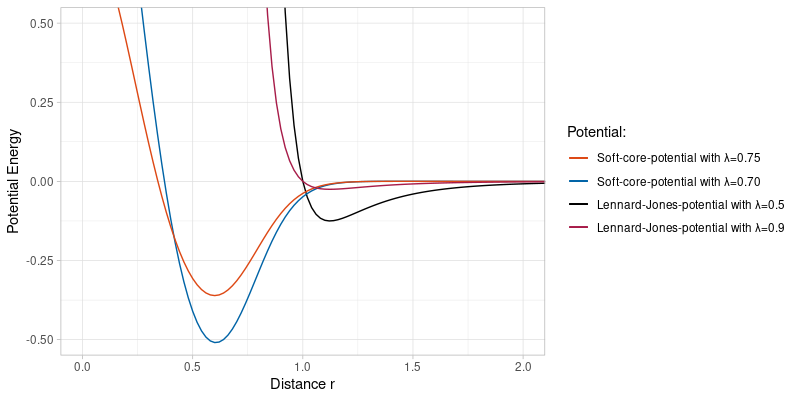
\includegraphics[height=6cm]{LJandsoftcore.png}
    \caption[Comparision between behaviour of standard LJ potentials vs. soft-core potentials]{Comparison between behaviour of standard Lennard-Jones and soft-core potentials for various states of $\lambda$. Visibly: For the standard LJ potential, well size decreases with increasing $\lambda$, while steepness of the potential wall increases. The reverse is true for soft-core potentials, which also remain defined at $r=0$}
    \label{fig:ljandsoftcore}
\end{figure}

To avoid this problem, soft-core potentials dependent on the coupling factor $\lambda$ were introduced as shown in Equation \ref{eq:ljsoftcore}\cite{Beutler1994Jun}:
\begin{equation}
U_{LJ}^{SC}(r,\lambda)=(1-\lambda)(\frac{A}{(r^2 +\lambda \delta)^6 }-\frac{B}{(r^6 +\lambda \delta)^3})
\label{eq:ljsoftcore}
\end{equation}
These mostly solve the problem, as there can now be no division by zero and the fractions remain finite in all circumstances. They are, however, computationally expensive  - especially for MD engines lacking native support for them\cite{Li2020Aug}. It is important to note that \texttt{Transformato} for this reason does \textbf{not} use soft-core potentials, but rather the "serial-atom-insertion" approach (see section \ref{sec:tf_principles}).


\section{The common-core serial-atom-insertion framework {\texttt{Transformato}}}
To avoid these problems and reduce general computational cost of FES, the common-core serial-atom-insertion framework \texttt{Transformato} was conceptualized and implemented. Being engine-agnostic - its outputs theoretically being computable with any of the widely-used Molecular Dynamics engines (openMM, CHARMM, AMBER, GROMACS, etc., though pre-provided simulation scripts are currently only available for CHARMM and openMM) - and provided as a python package, it allows straightforward calculation of relative binding and solvation free energy differences.


\subsection{Theoretical Principles} \label{sec:tf_principles}
\texttt{Transformato} is built on two distinct theoretical pillars: The \emph{Serial Atom Insertion} approach to generating intermediary states, and the \emph{Common-Core} approach to handling thermodynamic cycles, together referred to as the "serial-atom-insertion common-core" method (SAI/CC).

\emph{Serial Atom Insertion} (SAI)\cite{boresch_avoiding_2011} refers to an alternative method of avoiding the van-der-Waals-Endpoint problem without relying on the soft-core potentials discussed in section \ref{sec:vdwproblem}, developed by Boresch and Bruckner in 2011. This allows for a significant decrease of computational cost in MD engines without native, GPU-assisted soft-core modelling, at the drawback of having significant, stepwise changes to the states present in phase space, making it unsuitable for analysis via Thermodynamic Integration. Central to this method is to turn off the changed atoms in successive fashion, rather than scaling all of their interactions as one $\lambda$-dependent potential to generate the intermediate states. Thus, rather than depending on potentially very small $\lambda$ values (Eq. \ref{eq:nonsai} for the simplest case, outlined in section \ref{sec:intstatesanddummys}), the total potential energy is calculated by having the each atom turned on or off be its own intermediary state, with no intermediary scaling of the nonbonded parameters (Eq. \ref{eq:saipot}, for a molecule in solution with $M$ Lennard-Jones particles, itself containing $m$ particles with $u^{LJ}_{i,j}$ denoting the Lennard-Jones interaction between two particles).

\begin{equation}\label{eq:nonsai}
    U(\lambda)=\sum_{1\leq i<j \leq M} u^{LJ}_{i,j}+\lambda \sum_{1 \leq i \leq M} \sum_{1 \leq l \leq m} u^{LJ}_{i,j} \hspace{2cm} \lambda=[0,1]
\end{equation}
\begin{equation}\label{eq:saipot}
    U(k)=\sum_{1\leq i<j \leq M} u^{LJ}_{i,j}+\sum_{1 \leq i \leq M} \sum_{1 \leq l \leq k} u^{LJ}_{i,l} \hspace{2.3cm} k=[0,m]
\end{equation}

The \emph{Common Core} \cite{Wieder2022Jun,braunsfeldImplementationTestingCHARMM} on the other hand refers to the atypical alchemical path taken by \texttt{Transformato}. Whereas traditional FES transform the endstates directly into each other, \texttt{Transformato} instead transforms each of them into their maximum common topology - the \emph{Common Core}.This allows for significantly reduced computational time due to typically less intermediate states being required for the same precision \cite{Karwou2022Jun}, while avoiding complexity and room for error with e.g. selection of the reweighting function for TI.

Routing via the common core is useful, as the complete free energy difference between two ligands on the alchemical pathway (illustrated in Fig. \ref{fig:thermocycle_rbfe}) can be expressed as the sum of the individual free energy differences (Eq. \ref{eq:sumofligandtocc}).
\begin{equation}\label{eq:sumofligandtocc}
    A^{L_1\rightarrow L_2}_{bound}=\Delta \Delta G_{bound}^{L_1\rightarrow L_2}=\Delta \Delta G^{L_1\rightarrow [D_{L_1}]-R_{CC}}_{bound}-\Delta \Delta G^{L_2\rightarrow [D_{L_2}]-R_{CC}}_{bound}
\end{equation}
To reach the common core, a so-called \emph{mutation path} is generated by the program from each ligand $L_1, L_2$ to the CC $R_{CC}$, along which atoms not belonging to the CC are decoupled and transformed into dummy atoms. First, electrostatic interactions are turned off, followed by Lennard-Jones interactions of first hydrogen, then separately non-hydrogen atoms successively. The last atom connecting the \emph{dummy regions} $DL_1,DL_2$ with the CC is called the \emph{terminal junction} X, and is scaled linearly to have the bond specifications of $L_1$ match those of $L_2$. As the SAI/CC requires redistribution of charges\footnote{The sum partial charge of the terminal junction at the end needs to be 0 to cancel itself out across the thermodynamic cycle, see \cite{Karwou2022Jun,Wieder2022Jun} for details}, this atom retains some Lennard-Jones interaction and forms the anchor point for the dummy region. Each stage of this mutation forms an intermediary state similar to those used with $\lambda$-scaling methods, though not dependent on a numeric factor. After each intermediate state is simulated, $U_{i,j}$ may be calculated in postprocessing, allowing the calculation of free energy differences via mBAR. This is done both for the ligand in complex with the protein, as well as for the ligand in simple solution, allowing calculation of $A^{L_1\rightarrow L_2}_{bound}$ via exploitation of the cycle in Fig. \ref{fig:thermocycle_rbfe}.

It should be noted the two methods are independent from each other; it is quite possible to compute a direct transformation using SAI or to use the CC approach alongside soft-core potentials, with increasing adoption of native soft-core methods in MD engines making the latter especially a useful proposition. However, this is as of yet not implemented in \texttt{Transformato}.
\subsection{Theoretical considerations for Restraints in \texttt{Transformato}}
While \texttt{Transformato} yields excellent results for almost all test systems, problems may arise in unstable systems with a ligand prone to leaving the binding site of its associated protein within the timeframe of the simulation. This may even be a problem in comparatively stable systems, assuming a larger-than-usual timeframe is desired. To circumvent this, restraints need to be applied within the system, keeping the ligand within the binding site while still allowing sampling within it. However, irrespective of other considerations, the addition of restraints may not influence the calculated free energy differences, as this would render the entire exercise pointless. Restraints as implemented act as bonded force, and following Eq. \ref{eq:bondeds} are a simple addition to the sum forming $U_{bonded}$. Given that the free energy is directly dependent on $U$ via the partition functions (Eq. \ref{eq:nptpartition}) and the pathway energy results from the subtraction of the $L_2$ pathway from the $L_1$ pathway (Eq. \ref{eq:sumofligandtocc}), this means that $U^{restraints}_{L_1}$ must be equal to $U^{restraints}_{L_2}$ for the restraints to cancel each other out.

However, this is not possible for restraints involving the entire system. In case of a simple harmonic restraint as given by Eq. \ref{eq:simpleharmonic}), with $r$ the distance between the restrained particles - one anchored on the ligand, one anchored to the protein -, $r_0$ the equilibrium distance, and $k$ the force constant,  the amount of energy added to the system is proportional to the movement of the restrained systems vis-a-vis each other.
\begin{equation}\label{eq:simpleharmonic}
    U^{rest}=0.5\cdot k(r-r_0)^2 
\end{equation}
To achieve $\langle U^{rest}_{L_1}\rangle == \langle U^{rest}_{L_1}\rangle$, the first condition is the same number of restraints in the system. However, as $\langle U \rangle$ is dependent on $r$, the expectation value for $r$ may also not change. As $r$ is dependent on the atom interactions and thus its given force field parameters, that means that the restraint needs to be connected to the same atom types (or groups of atom types) at both endstates. The current implementation in \texttt{Transformato} achieves this by restricting its restraints to the common core, as that represents a useful list of atoms that will both remain constant during the mutations and have the same atom type in both ligands, barring the terminal junction.

However, the common core does not exist in a vacuum, and $r$ is dependent not only on movement by the ligand, but that of the protein as well. To satisfactorily keep ligands restrained in the binding site while still allowing for low enough force constants to facilitate sampling, current automatic restraints anchor to protein carbon-alphas near the ligand. These are affected by the ligand, with different ligand structures producing different effects. These differing interactions will also have differing effects on the movement of the common core structures, further diverging $\langle (r-r_0) \rangle$ between $L_1$ and $L_2$. While the anchoring of the restraints exclusively to alpha carbons is an attempt to minimize this and contributions are likely to be small, is is nevertheless an inaccuracy introduced into the calculations.

To minimize this inaccuracy, restraints may simply be turned of for the endstates. With mBAR, as the $\hat{A}_i$ is formed from the sum differences between two adjacent states (Eq. \ref{eq:bar_freeenergy}), as long as the restraints are introduced away from the endstates, their energy contribution is considered in $\Delta \hat{A}_{1}\rightarrow \hat{A}_{2}$ at both sides instead of being part of the initial system. As the contribution at the common core is necessarily the same, the terms thus cancel each other out. \texttt{Transformato} provides the keyword \code{scaling} for this, which scales $U^{restr}$ linearly across the first four intermediary states, with the endstates receiving no contribution at all.

On the topic of contribution, harmonic restraints as in Eq. \ref{eq:simpleharmonic} suffer the disadvantage of always having a contribution to the total potential, as given the high numerical precision of simulations along with initial velocities assigned at the start of the system means that $r-r_0$ never evaluates to 0. Similarly, the harmonic shape of the restraint means that a restraint capable of stopping escape from a binding site will have significant contributions even within that binding site, discouraging sampling and possibly introducing errors into the energy calculations that way. To alleviate this, it is recommended to instead use flat-bottom potentials as in Eq.\ref{eq:flatbottom}.
\begin{equation}\label{eq:flatbottom}
    U^{rest}=k \cdot step(|r-r_0|-wellsize) \cdot (r-r_0)^2
\end{equation}
With $r$ once again representing distance, $r_0$ being the equilibrium distance and $k$ the force constant. New additions are the $wellsize$ and a $step$ function. The wellsize represents a radius around the equilibrium distance which the restraint is free to move around in. As long as the expression $|r-r_0|-wellsize$ evaluates negative, $step(x)=0$. Should it however evaluate positive, meaning that the restraint has left the well, the step function evaluates to 1 and the standard harmonic restraints are applied. This allows definition of fairly stringent restraints without impact on sampling within the binding site.
\subsection{Usage}
Installing \texttt{Transformato} is fairly straightforward: it requires a working installation of \texttt{conda} and \texttt{python}. Using \texttt{git clone}, download the package from the repository\footnote{\url{https://github.com/JohannesKarwou/Transformato}} and run \texttt{python setup.py install}. This will install a conda environment called \texttt{fep} consisting of \texttt{Transformato} and all its dependencies. Activate the environment and you're done.

To calculate free energies, retrieve a PDB containing your ligand-protein complex for both endpoints. For each, solvate once the complex including the ligand and once just the ligand using e.g. CHARMM-GUI's Solvation Builder\footnote{\url{https://www.charmm-gui.org/}}. Take the output folders, equilibrate them and name the 'complex' and 'waterbox', respectively. You will then need to create a config.yaml file containing the names of your structures and parameters you want your simulation to have - any restraints you wish to apply must also be defined here. The simplest case for specifying restraints is simply done by adding the keyword \code{restraints: auto} to the \emph{simulation} part of the configuration file. This restrains the entire ligand backbone via its center of mass to the center of mass of the protein backbone. Inside the code, this is referred to as \texttt{simple} mode. Another possibility is the generation of restraints on the extremities of the ligand using the \code{extremities=[int]} keyword. This algorithmically selects those carbon atoms furthest from the center of mass (and each other), and restrains these and their surroundings to the protein, thus cutting down on rotational freedom. The downside of this is that it requires some prior knowledge of the ligand's shape - not usually a problem, but potentially in large-scale applications. Of course, this also reduces sampling volume even further than the simple restraint. Lastly, it is also possible to manually define restraints in addition to - or instead of - the automatic ones, using the keyword \code{restraints: manual} and defining manual restraints below. This allows full use of the MDAnalysis\cite{agrawal2011,oliver_beckstein-proc-scipy-2016} selection syntax, limited only by the common core on the ligand.

\begin{figure}[h]\small

\begin{verbatim}
Free energy to common core: 12.02382 [kT] with uncertanty: 0.5843413703 [kT].
Free energy difference: 12.02382 +- 0.584341 [kT]
Both states are considered
\end{verbatim}
\label{fig:anaoutput}
\caption{Typical output of analysis.py}
\end{figure}

To actually create the simulation runs, you will need a modified 'submit.ipynb. These files sequentially load the .yaml config and the structure topologies, then propose a common core. After this point, you may add (or remove) atoms from the common core. Afterward, \texttt{Transformato} will propose a mutation route. If it looks satisfactory, it will then create several folders containing intermediate states, each a self-contained simulation. Simulate these (as this is the most computationally intensive step, it is highly recommended to use a cluster for this step) and run the analytics script (a cluster is also recommended here). In the end, you should receive output similar to Figure \ref{fig:anaoutput}. Please note that the energy difference to the common core is usually only one leg of the journey; unless one of the endstates is identical to the common core, you will need to add the values for both to get the actual relative free energy. 

Significantly more extensive documentation of \texttt{Transformato}'s abilities and features is available through the GitHub repository wiki at \url{https://github.com/JohannesKarwou/Transformato/wiki}, along with sample input and data files.


\chapter{Methods}
\section{Implementation of restraints into \texttt{Transformato}}

The process of applying restraints was divided into four parts:

\begin{enumerate}
    \item Processing user input: the general demand for restraints, and parameters for these restraints
    \item Finding suitable binding sites and generating the atom selections for the restraints
    \item Generating an openMM Force object
    \item Applying this Force to the actual simulation

\end{enumerate}

These processes were complicated by the fact that the script that generates the intermediate states for processing (and thus has access to user input) is separate from those that do the actual simulations (which need to be independent to be able to run on distributed computing networks).



 As much code as possible was exiled into a separate module file called \code{restraints.py}, with only minimal changes to \code{state.py} and \code{mutate.py} being necessary. 

Currently, restraints are only available as a proof-of-concept for openMM. OpenMMs \emph{CustomCentroidBondForce} was chosen as basis for all restraints. To facilitate analysis of Ligand and Protein structures, MDAnalysis\cite{agrawal2011,oliver_beckstein-proc-scipy-2016} was used.

\subsection{Processing user input}
To leverage the existing codebase as well as keeping with the established design principles of \texttt{Transformato}, additional user input was restricted to the configuration \texttt{.yaml} already required; to ensure both backward compatibility and prevent accidental use of restraints all commands to use restraints are purely optional. If a user is unaware of the possibility of restraints, they will not run into the danger of accidentally using them. Further, there is no additional workflow in the users' submit script - all of it is done during \code{utils.py::load\_config\_yaml()} automatically.

Due to the structure of the existing code, no changes to \code{utils.py} were necessary - all relevant information was available for further processing immediately.
\subsection{Finding suitable restraints}

\subsection{Generating an openMM Force object}

\subsection{Applying the Force to the actual simulation}
\section{RBFE calculations}
All inputs were generated using CHARMM-GUI\cite{Jo2008Aug}, and used the CHARMM36m forcefield\cite{Huang2017Jan}. For easier handling and allowing larger timesteps, CHARMM-GUI's facility for hydrogen mass repartitioning\cite{Gao2021Feb} was used unless noted. Equilibration was done using the openMM - Inputs provided by CHARMM-GUI\cite{Brooks2009Jul,Lee2016Jan}. To modify the ligand, CHARMM-GUI's ligand designer\cite{Guterres2021Nov} was used alongside the commercial program Maestro\cite{maestro}. The simulations themselves were carried out using openMM 7.5\cite{Eastman2017Jul}


\subsection{2OJ9 - Tautomer A with modified BMI}
\begin{figure}[H]
    \centering
    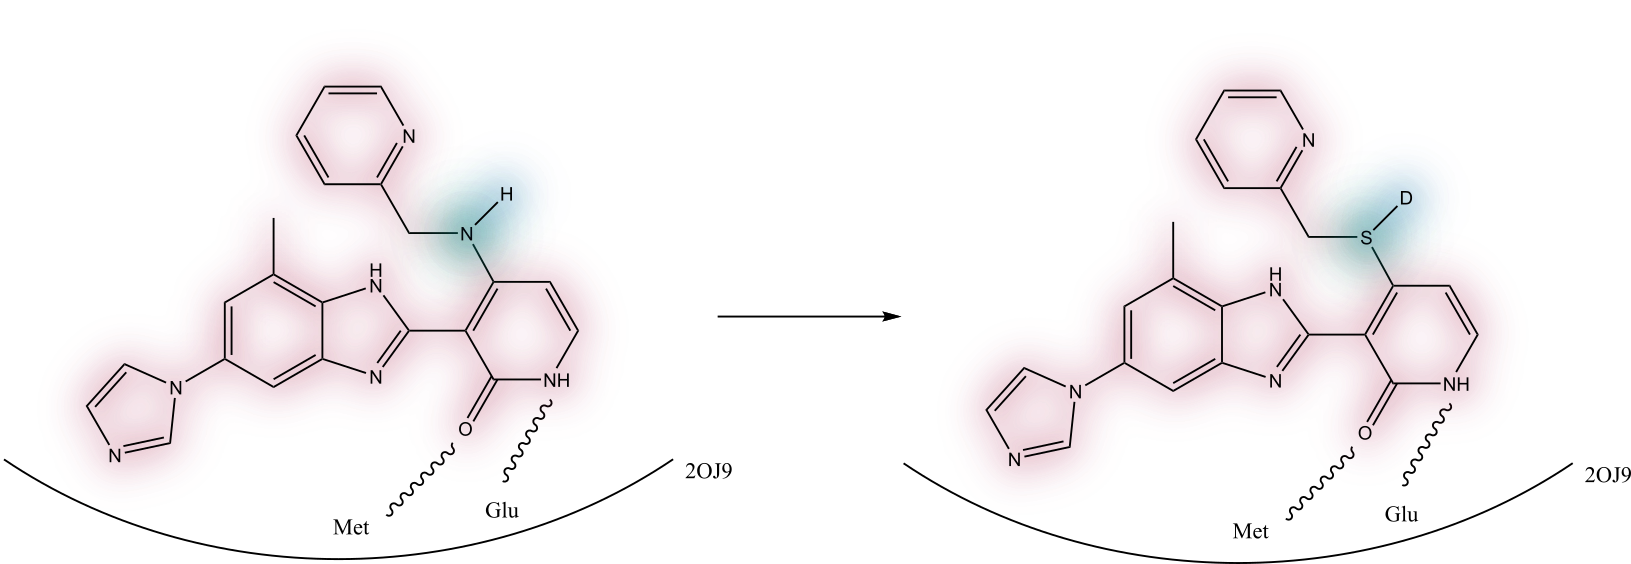
\includegraphics[width=\textwidth]{taapdb24to25.png}
    \caption{2OJ9 Tautomer A, with functional groupings shaded. Red: common core. Green: terminal X. Blue: dummy region. Of note: the two likely bonds to the protein.}
    \label{fig:2oj9_struc_taapdb}
\end{figure}
\subsection{2OJ9 - Tautomer B with modified BMI}
\subsection{Vim2: ZN148 relative to ZN223, ZN222 and ZN228}
Vim2 is a Carbapenem-Hydrolyzing Metallo-$\beta$-Lactamase, responsible for a subtype of bacterial drug resistance.\cite{Poirel2000Apr}. ZN148 and ZN223 are specific zinc ligands first presented by Samuelsen et al.\cite{Samuelsen2020Jun}. These ligands are designed to inhibit Vim2 activity and suppress its drug-resistant activity, thus providing a treatment vector for strains containing it. 

To prepare the structures for use in transformato, protonation states were determined by use of ProToss\cite{Lippert2009Dec,Bietz2014Dec} and manual observation, after which ligand and protein were solvated using CHARMM-GUI's solvation builder, including patching of the C-Terminus. As certain binding modes require the presence of an OH$^-$ group nearby, but CHARMM-GUI's solvation builder is unable to process the system with it, a roundabout way was chosen where a separate .crd file for the OH group was created and patched in after solvation using \texttt{macha}\cite{twotoneblue2022May}. As this also complicated HMR, Hydrogen Mass Repartitioning was accomplished using \texttt{parmed}\cite{Shirts2016Sep}. Afterwards, use in \texttt{Transformato} continued as normal.



\chapter{Results}
To test both the successfull application of the restraints, and their impact on calculated RBFE, a number of simulations were conducted using test systems 2OJ9 and VIM2. \textbf{It should be noted that the energies calculated here do not represent actual free energies}, as all simulations were conducted from one physical endstate to the common core; while the systems were chosen in a way that the common core topology is identical to the second physical endstate, this is not an acceptable substitute for caluclating the energy difference for both mutation routes. However, the goal of these simulations was simply to serve as instructive checks whether the main goals of the work (introduction of restraints) had been achieved and whether those had significant impact on calculated $ \Delta \Delta G$. All results are averaged from runs with three replicates.
\section{Application of restraints to classical MD simulations}

To verify the validity of the general approach, a variety of restraints were introduced to 2OJ9 systems outside of \texttt{Transformato}, and simulated with standard MD for ten nanoseconds. Afterwards, trajectories were analyzed with regard to the distance between the supposed binding sites to the protein, as well as root mean square deviation and potential energy.
\section{Application of restraints to \texttt{Transformato} RBFE calculations}
\newpage
\subsection{2OJ9: Tautomer A of BMI, 24 to 25}

\begin{table}\small
\begin{center}
    \begin{tabular}{l|r|l|r|r}
        Restraints & k - value & scaling & Average [kT] & SD [kT]   \\
        \hline
        Extremities & 100 & no  & -1.15 & 2.15                                   \\
        Extremities & 100 & yes & 0.11  & 1.95                                   \\
        Simple      & 100 & no  & 0.09  & 1.22                                   \\
        Simple      & 100 & yes & -0.97 & 0.41  \\
        Extremities & 10  & no  & -1.87 & 0.04   \\
        Extremities & 10  & yes & -1.30 & 1.69                                   \\
        Simple      & 10  & no  & 0.30  & 1.45                                   \\
        Simple      & 10  & yes & -0.74 & 0.77   \\
        Extremities & 3   & no  & -0.35 & 1.73                                   \\
        Extremities & 3   & yes & 0.27  & 1.00                                   \\
        Simple      & 3   & no  & -1.82 & 0.50   \\
        Simple      & 3   & yes & -2.05 & 2.61                                   \\
        Extremities & 400 & no  & 1.11  & 2.89                                   \\
        Extremities & 400 & yes & 5.39  & 1.31                                   \\
        None        & N/A & no  & -1.07 & 1.08                                  
    \end{tabular}
\end{center}
\caption{2OJ9 Tautomer A, $\Delta\Delta G_{bind}L_{24}\xrightarrow{} L_{25}$. Simulation Time: 1.25 ns, Step Time: 1fs, 3 Replicates}
\label{tab:2oj9_taapdb_24to25_shortruns}
\end{table}

\begin{table}\small
\begin{center}
\begin{tabular}{l|l|l|l|l|}
Restraints & k- value & scaling & Average [kT] & SD [kT]\\
\hline
Simple   & 400 & yes & 9.52  & 0.99 \\
Simple & 400 & no  & 9.40  & 1.34 \\
Extremities      & 400 & yes & 8.20  & 1.61 \\
Extremities       & 400 & no  & 10.34 & 0.99 \\
Simple    & 100 & yes & 8.29  & 0.86 \\
Simple  & 100 & no  & 10.10 & 0.21 \\
Extremities         & 100 & yes & 9.36  & 1.45 \\
Extremities       & 100 & no  & 10.24 & 2.33 \\
Simple   & 10  & yes & 8.63  & 0.38 \\
Simple    & 10  & no  & 9.42  & 2.61 \\
Extremities          & 10  & yes & 9.80  & 0.98 \\
Extremities        & 10  & no  & 10.98 & 1.35 \\
Simple     & 3   & yes & 10.00 & 0.41 \\
Simple    & 3   & no  & 9.88  & 1.28 \\
Extremities         & 3   & yes & 9.33  & 1.92 \\
Extremities         & 3   & no  & 9.43  & 1.17 \\
None & N/A & no & 8.77 & 1.85
\end{tabular}
\end{center}
\caption{2OJ9 Tautomer B, $\Delta\Delta G_{bind}L_{24}\xrightarrow{} L_{25}$. Simulation Time: 1.25 ns, Step Time: 1fs, 3 Replicates}
\label{tab:2oj9_tablit_24to25_shortruns}
\end{table}


\chapter{Discussion}

\section{Comparison to experimental results}
\section{Future possibilities }
\chapter{Annex}
\section{Definitions}
As far as possible, equations in this thesis are notated and styled as in the Alchemistry Wiki maintained by Shirts and Chodera \cite{shirts_alchemistrywiki_nodate}. The symbols and notations used resolve as follows:
\begin{center}
    

\begin{tabular}{ | m{3cm} | m{10cm}| }
\hline
$Q$ & the partition function of the canoncial ensemble \\
\hline
$k_B$ & Boltzmann's constant\\
\hline
$T$ & Temperature \\
\hline
$P$ & Pressure \\
\hline
$V$ & (Box) Volume\\
\hline
$U$ & Sum of internal energy in a MD simulation, both potential and kinetic energies\\
\hline
$N$ & Number of particles in the system\\
\hline
$\beta$ & Substitute for $(k_B T)^{-1}$ by convention \\
\hline
$\Gamma$ & Phase Space Volume \\
\hline
$\lambda$ & the \emph{alchemical variable} or \emph{coupling parameter}. Used to describe the progress of a transformation along the alchemical path\\
\hline
$K$ & The \emph{state variable}, describing all conditions and parameters of the thermodynamic system\\
\hline
$k$ & A specific state found in $K$\\
\hline
$u$ & The \emph{reduced potential} $u=\beta(U+PV-\sum{\mu N_i}) $. For NPT ensembles, $\sum{\mu N_i} = 0$\\
\hline
\end{tabular}
\end{center}
\listoffigures

\listoftables

\printbibliography[title={References}]%heading=subbibnumbered,
\end{document}